\section{Twisted Pair/Coaxial Cable}
\frame{
\frametitle{\secname
\footnote{Disclaimer: I am not an Electrical Engineer}}

\begin{columns}
\column{0.5\textwidth}
\begin{itemize}
\item<1-> Electric current makes magnetic fields
\item<1-> Excessive magnetic fields causes noise and interference
\item<1-> Idea: place reverse current close to forward current to have fields cancel
\item<1-> Twisted pairs!
\item<2-> To make the fields align and cancel even more, the two conductors can be made to share the same axis
\item<2-> Coaxial cable!
\end{itemize}

\column{0.5\textwidth}
\only<1>{
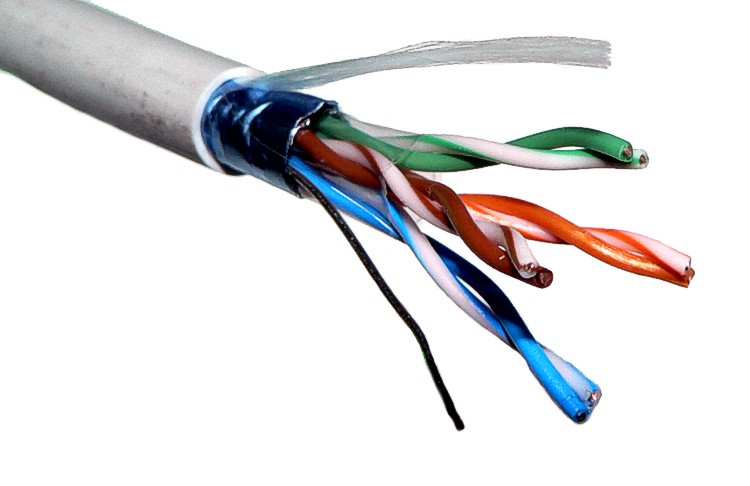
\includegraphics[width=0.9\textwidth]{slides/twistedpair_coax/FTP_cable3.jpg}
}
\only<2>{
\includesvg[width=0.9\textwidth]{slides/twistedpair_coax/Coaxial_cable_cutaway.svg}
}
\only<3>{
\begingroup
\sbox0{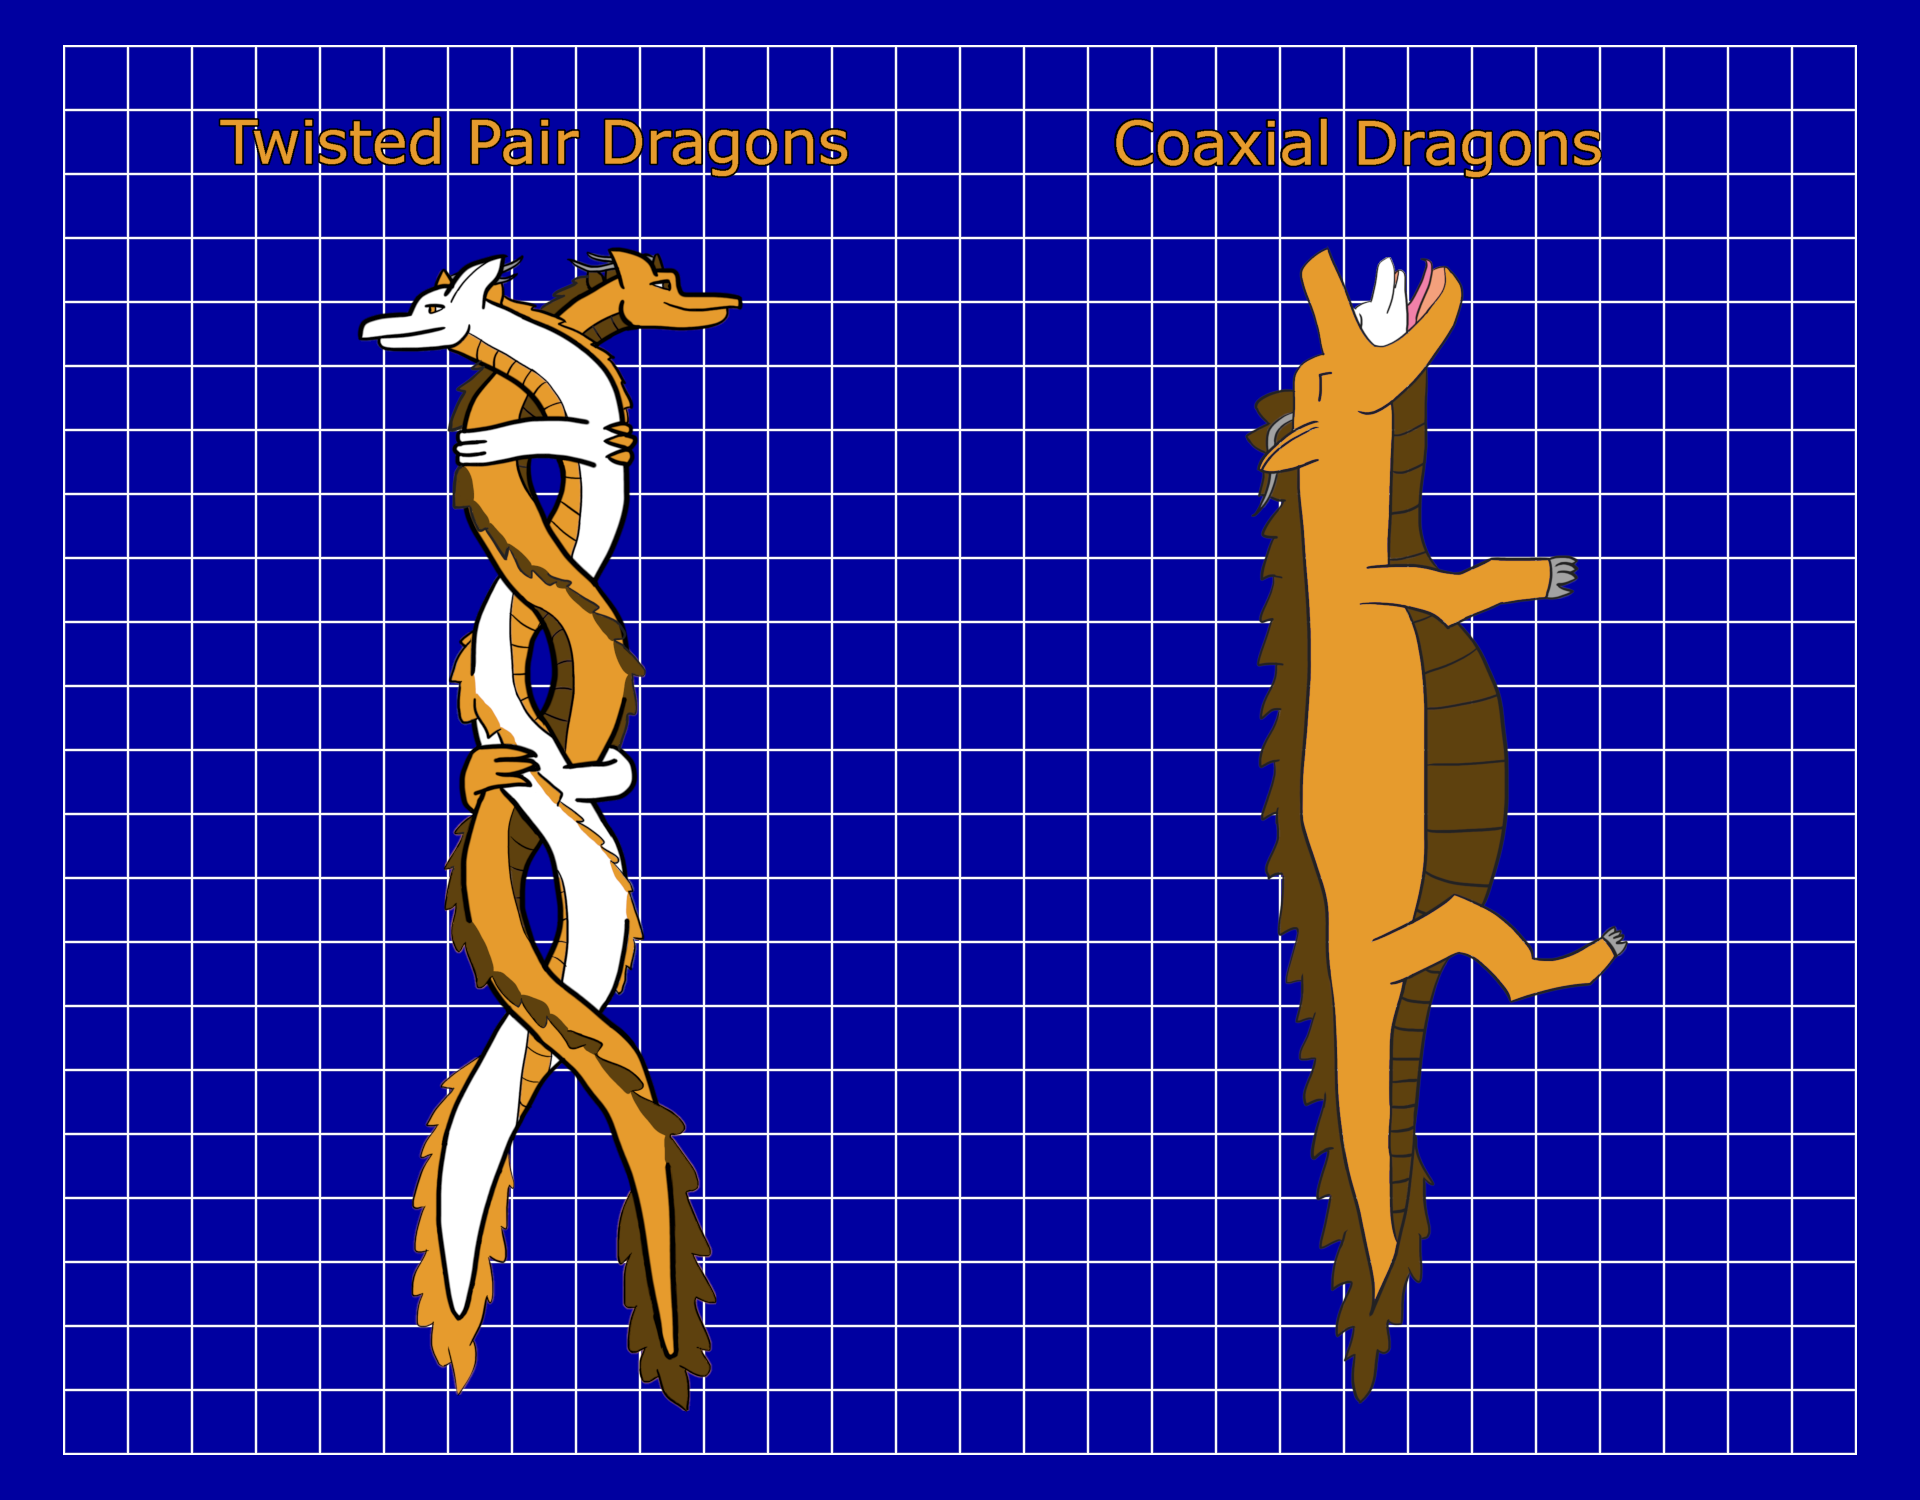
\includegraphics{slides/twistedpair_coax/TwistedPairCoax.png}}%
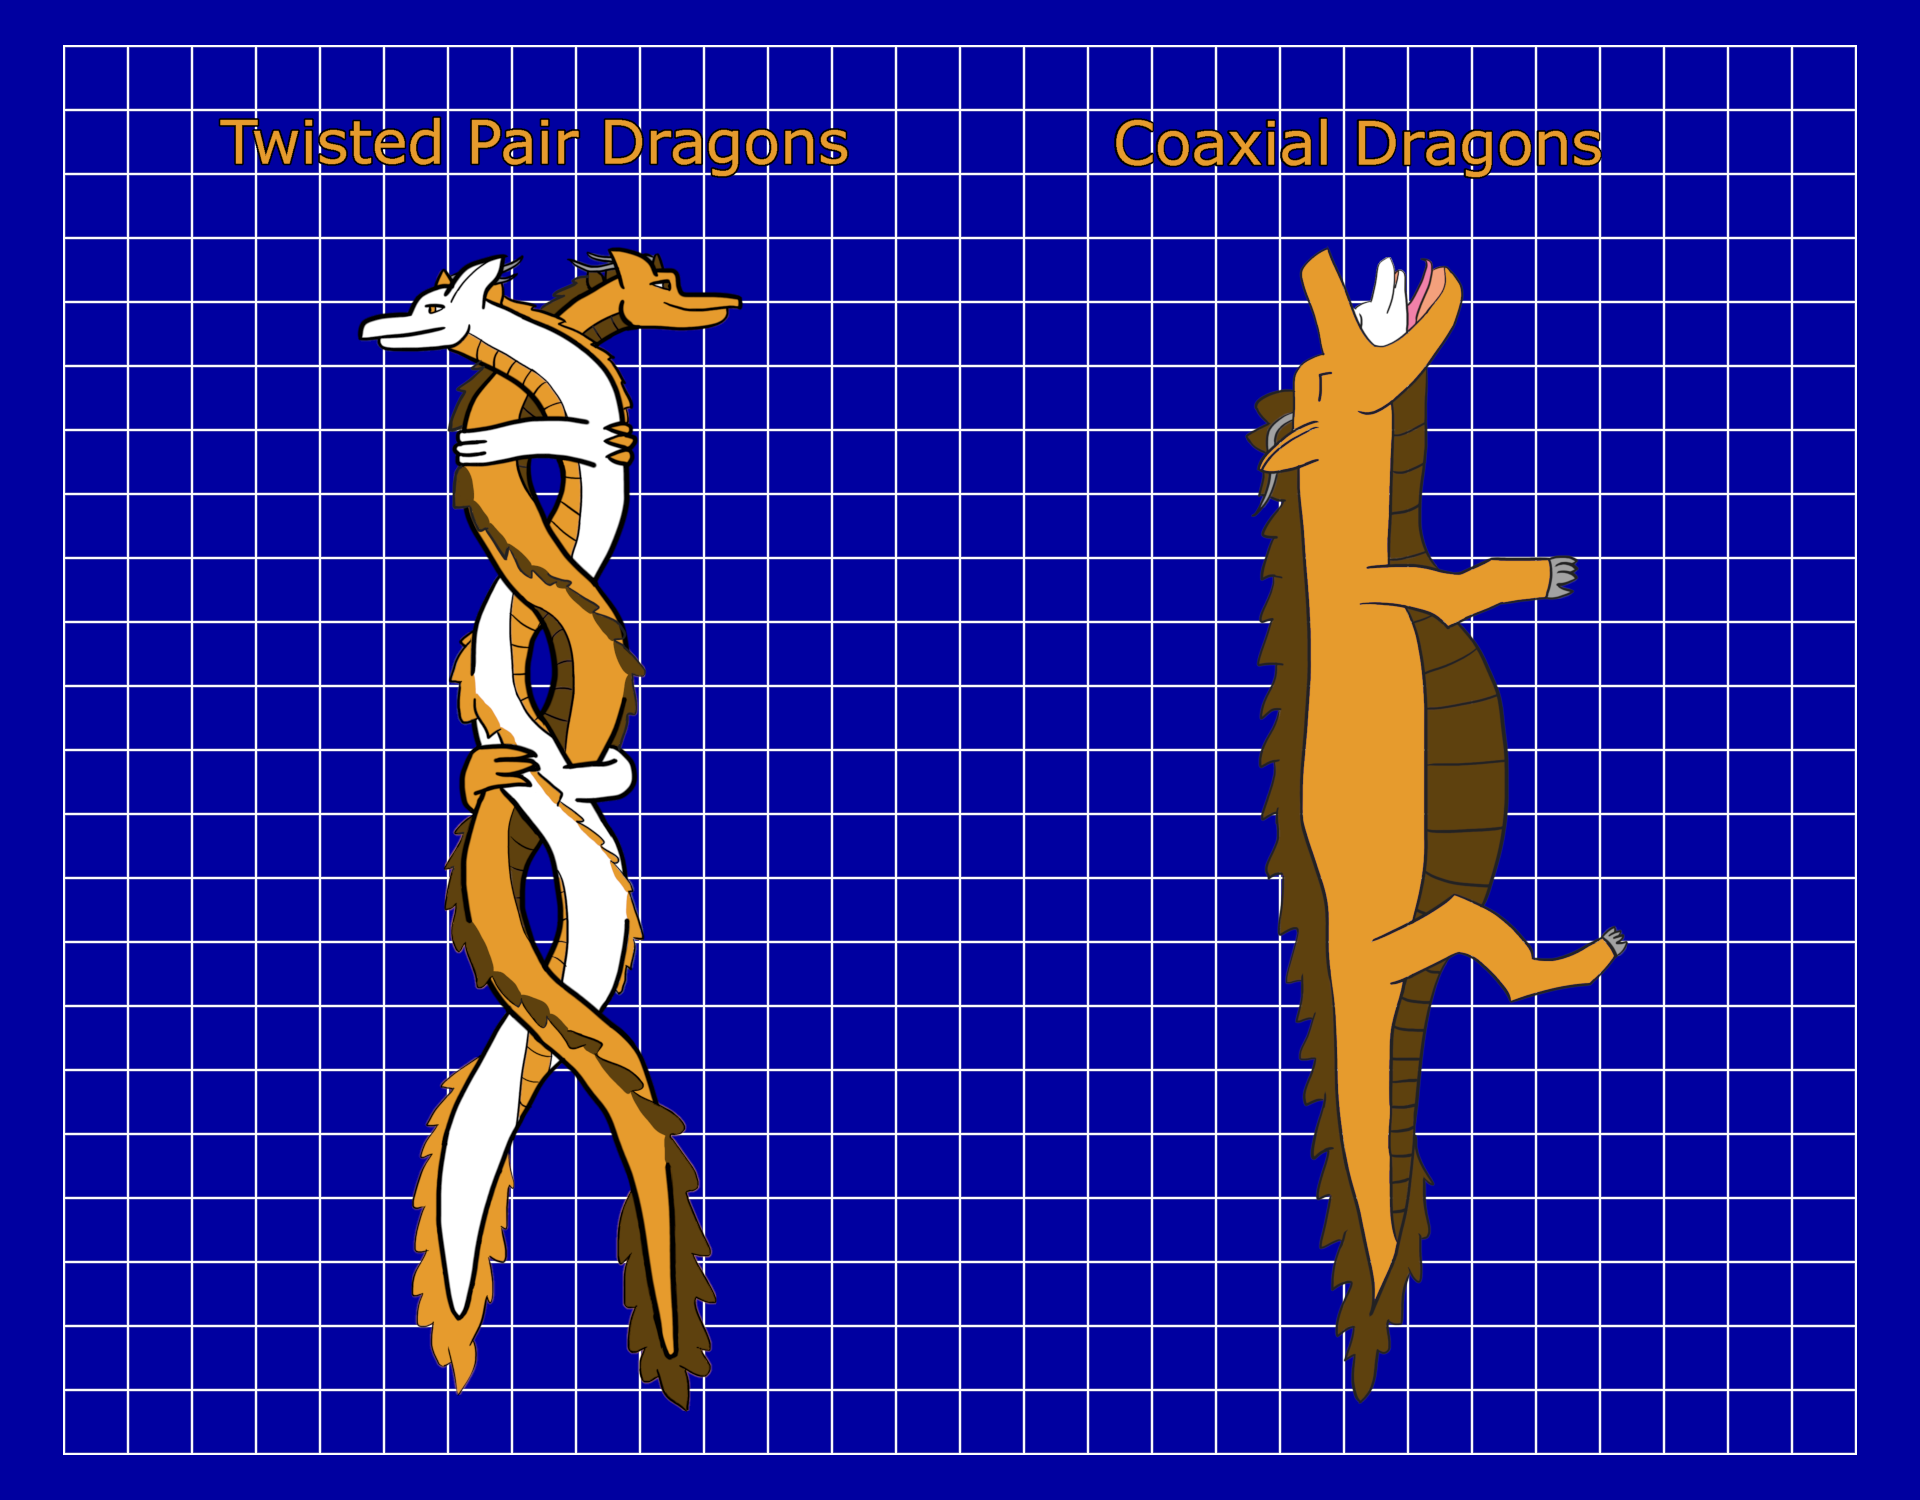
\includegraphics[clip,trim=0 0 {.5\wd0} 0,width=.45\textwidth]{slides/twistedpair_coax/TwistedPairCoax.png}
\endgroup
}
\only<4>{
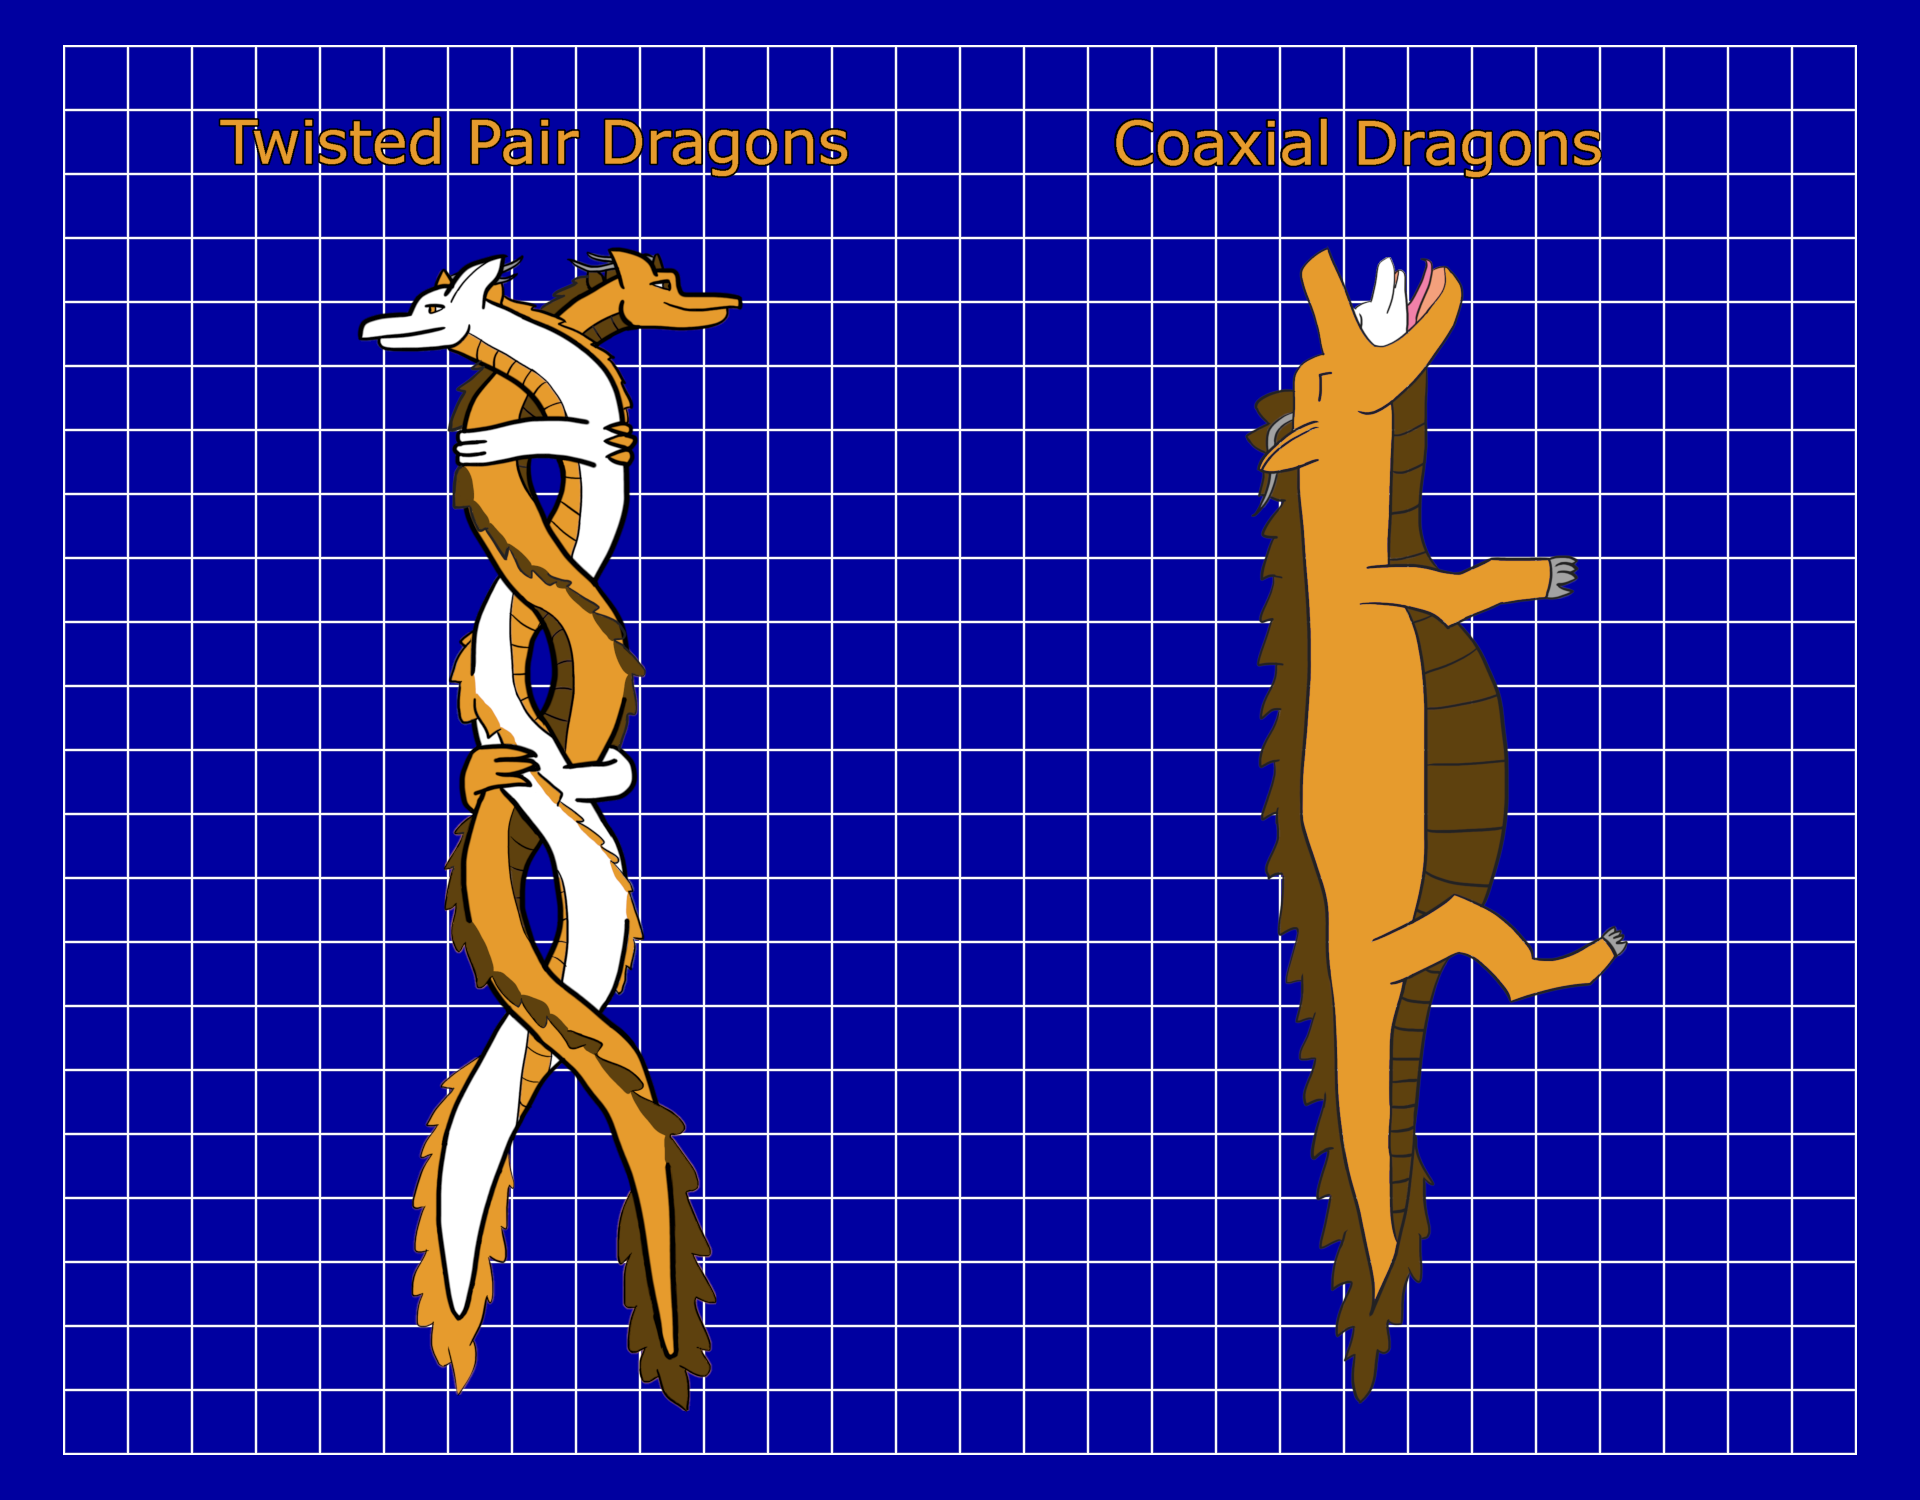
\includegraphics[width=0.9\textwidth]{slides/twistedpair_coax/TwistedPairCoax.png}
}

\end{columns}
}